\section{SBG V8: Evidence Model and Decision Procedure}\label{sec:approach}

\subsection{Architecture Overview}
Fig.~\ref{fig:architecture} shows the components of \sbg{} and Fig.~\ref{fig:pipeline} the path from a change to a verdict. \sbg{} is built around its predecessor, the V7-B differential engine, which it runs unmodified: the engine executes $P$ and $P'$ on each input in a fresh sandboxed child process, compares canonical observations, and issues a V7-B verdict through a fixed sufficiency gate. \sbg{} adds four layers around it: (i)~parent-side capture of per-input line and branch hits and of an independent copy of standard output (Section~\ref{sec:trust}); (ii)~sealing and validation of the resulting evidence directory; (iii)~a profile $\prof$ and a calibrated risk model that replace the fixed gate; and (iv)~the \ers{} audit, which perturbs evidence and records how the risk and the verdict respond (Section~\ref{sec:ers}). The implementation is in Python; it executes Python programs at function granularity.

\begin{figure*}[!t]
\centering
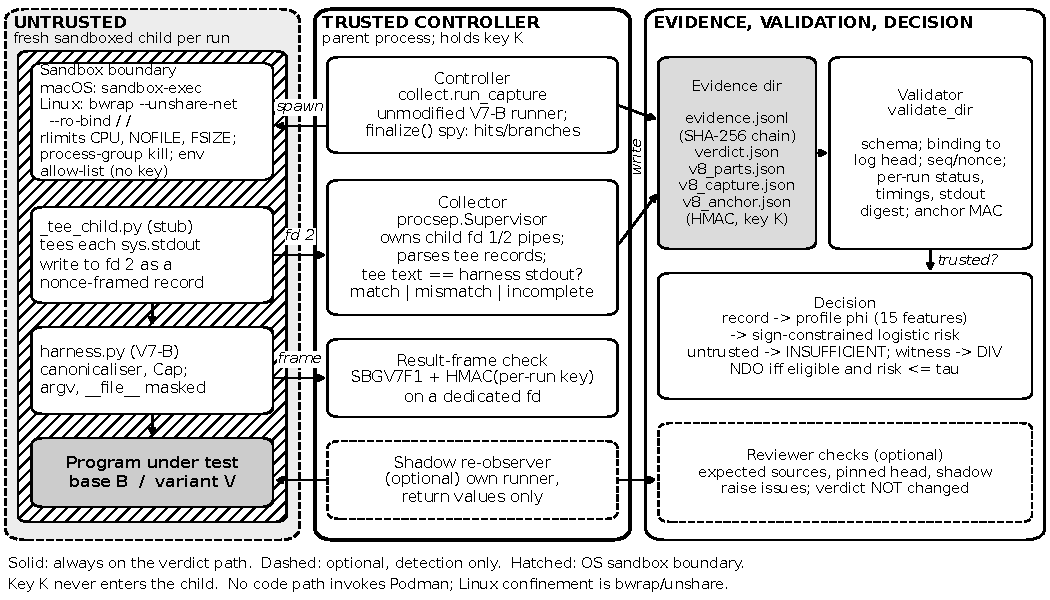
\includegraphics[width=\textwidth]{figures/fig_architecture.pdf}
\caption{\sbg{} architecture as implemented. The program under test runs in a fresh sandboxed child per run (macOS \code{sandbox-exec}; Linux \code{bwrap} with network unsharing). The trusted controller holds the anchor key $K$, which never enters the child, captures an independent tee of standard output, and checks the HMAC-authenticated result frame. Validation of the sealed evidence directory gates the verdict; shadow re-observation and source binding are optional reviewer checks that report issues but do not change the verdict.}
\label{fig:architecture}
\end{figure*}

\begin{figure}[!t]
\centering
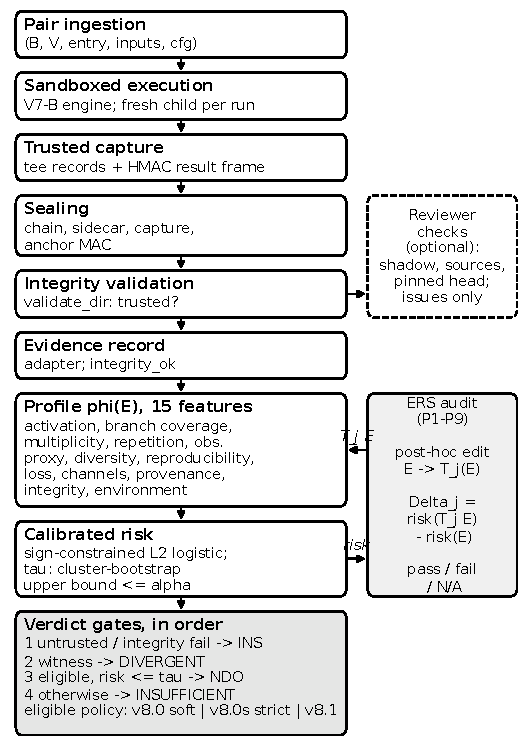
\includegraphics[width=0.92\columnwidth]{figures/fig_pipeline.pdf}
\caption{Evidence-to-verdict pipeline. The \ers{} audit applies a perturbation $T_j$ to a copy of the evidence record and compares the estimated risk before and after; it never modifies the original evidence.}
\label{fig:pipeline}
\end{figure}

\subsection{Change-Conditioned Evidence Profile}
The profile is \emph{change-conditioned}: every quantity is computed relative to the changed units $U_c$ rather than to the program as a whole. Let $C\subseteq I$ be the \emph{clean} inputs: non-duplicate inputs whose outcome is \code{SAME}, that are deterministic and that are not lossy. For an input $i$ let $h(i)$ be the changed units it executed and $\textit{fp}(i)$ its observation fingerprint (an input without a fingerprint is never treated as equal to another). Table~\ref{tab:profile} lists the fifteen features. The central ones are:

\emph{Activation}, the share of changed units executed by clean inputs,
\begin{equation}
a(\Ev) = \frac{\left|\bigcup_{i\in C} h(i)\right|}{|U_c|}.
\label{eq:act}
\end{equation}

\emph{Multiplicity}, the number of observationally distinct clean inputs that reached each changed unit,
\begin{equation}
\mu_u = \left|\{\textit{fp}(i) : i\in C,\ u\in h(i)\}\right|, \qquad \mu_{\min}=\min_{u\in U_c}\mu_u .
\label{eq:mu}
\end{equation}
Multiplicity is the feature that separates ``the change was reached'' from ``the change was reached in several observably different ways''. Counting fingerprints rather than inputs makes it insensitive to repeated identical observations.

\emph{Effective diversity} $n_{\textit{eff}}$, the number of distinct fingerprints among clean inputs, and its provenance-qualified variant, which counts distinct (fingerprint, provenance) pairs among inputs whose provenance is trusted and not derived from labels.

\emph{Reproducibility, loss and channels}: the share of deterministic inputs, the share of lossy or degenerate observations, and the mean fraction of declared channels actually captured per input.

\emph{Gate features}: provenance, integrity and environment consistency, each a binary indicator.

\begin{table}[!t]
\caption{Evidence profile $\prof(\Ev)$ as implemented (\code{sbgv8/profile.py}). Count features enter the model as $\log(1+x)$. ``Const.'' marks features that were constant on the development corpus and therefore carried no information there.}
\label{tab:profile}
\centering
\scriptsize
\setlength{\tabcolsep}{3pt}
\begin{tabular}{|L{2.3cm}|L{3.4cm}|L{1.5cm}|}
\hline
Feature & Definition & Dimension \\
\hline
\code{act\_frac} & Share of $U_c$ executed by clean inputs, Eq.~\eqref{eq:act} & Activation \\
\code{branch\_cov\_min} & Min.\ over sides of observed branch directions on changed lines, relative to $2\times$ static branches & Coverage \\
\code{mu\_min}, \code{mu\_mean} & Min.\ and mean of $\mu_u$, Eq.~\eqref{eq:mu} & Multiplicity \\
\code{n\_same} & $|C|$ & Quantity \\
\code{n\_rep} & Total repeat, replay and alternative runs over $C$ & Repetition \\
\code{obs\_react} & Share of $U_c$ reached by a clean, non-degenerate input with at least one captured channel (a \emph{reachability proxy} for observable influence, not a dependence analysis) & Influence \\
\code{n\_eff} & Distinct fingerprints in $C$ & Diversity \\
\code{n\_eff\_prov} & Distinct (fingerprint, provenance) pairs with trusted provenance & Diversity \\
\code{repro\_frac} & Share of deterministic inputs & Reproducibility \\
\code{lossy\_frac} & Share of lossy or degenerate inputs & Loss \\
\code{chan\_complete} & Mean share of declared channels captured & Channels \\
\code{prov\_ok} & All inputs have trusted, non-label-derived provenance (const.) & Provenance \\
\code{integrity\_ok} & Evidence passed validation (const.) & Integrity \\
\code{env\_ok} & Environment consistent across runs (const.) & Environment \\
\hline
\end{tabular}
\end{table}

Two limitations of the profile matter for interpreting the results. First, the observable-influence feature is a reachability proxy: it records that a changed unit was reached by an input whose output was captured, not that the unit's effect propagated to that output; dynamic dependence or checked coverage~\cite{schuler2011assessing} would be the principled replacement. Second, on evidence collected by the current adapter, provenance and environment are not populated from the runs and default to ``trusted'' and ``consistent'', and every development record passed integrity validation. These three features were therefore constant on the development corpus; their effect is examined only through the perturbations P7--P9.

\paragraph*{A profile defect found by \ers{}} In the version evaluated on the Linux branch, quantity and diversity features were computed over all non-duplicate inputs, including inputs that reached no changed unit and unflagged copies of the same observation. Irrelevant inputs could therefore raise $n_{\textit{same}}$, $n_{\textit{rep}}$ and $n_{\textit{eff}}$. This defect was exposed by perturbation P2 (Section~\ref{sec:results}) and fixed by restricting all features to \emph{relevant} evidence---inputs that reach at least one changed unit---and by collapsing unflagged copies into one evidence class. All statistical results are reported for the pre-fix profile, with the effect of the fix stated alongside.

\subsection{Verdict Logic}
Verdicts are produced by three layers applied in order.
\begin{enumerate}
\item \emph{Trust gate.} If validation of the evidence directory fails, or integrity is violated, the verdict is \INS{}; untrusted evidence can produce neither \NDO{} nor \DIV{}.
\item \emph{Witness.} If any input has a confirmed, reproducible divergence, the verdict is \DIV{}.
\item \emph{Calibrated abstention.} If the evidence is \emph{eligible} and $\Rhat(\Ev)\le\tau$, the verdict is \NDO{}; otherwise \INS{}.
\end{enumerate}
Eligibility is defined by a blocker policy over the reason codes that V7-B records when it would abstain (no clean input, unobservable outcome, nondeterminism, changed region not activated, budget exhausted, environment sensitivity). Under the \emph{soft} policy (v8.0) only the blockers ``changed region not activated'' and ``budget exhausted'' are tolerated, so that activation becomes a graded feature rather than a hard gate. Under the \emph{strict} policy (v8.0s) no blocker is tolerated, and under v8.1 the record must additionally be one on which V7-B itself would issue \NDO{}. On the development corpus, v8.0s and v8.1 select the same set. Under the strict policies the calibrated model can only abstain further within V7-B's own \NDO{} set.

\subsection{Change-Conditioned Evidence Calibration}
The risk model $g$ is an $L_2$-penalised logistic regression of the label on the standardised profile, fitted on eligible labelled pairs only. Sign constraints declared before fitting encode domain knowledge: every evidence feature may only lower the estimated risk, except the loss share, which may only raise it. The constraints are enforced as box bounds in L-BFGS-B. The penalty $\lambda\in\{0.3,1,3,10\}$ is chosen by inner project-grouped three-fold cross-validation on log loss. In the full \cec{} model the nine \ers{} responses $\Delta_j$ (Section~\ref{sec:ers}) enter as additional features with free sign.

The threshold $\tau_\alpha$ for a target risk $\alpha$ is chosen on inner out-of-fold predictions: eligible pairs are ranked by $\Rhat$, and $\tau_\alpha$ is the largest score whose prefix has a one-sided 95\% project-cluster bootstrap upper bound on selective risk not exceeding $\alpha$. If no prefix qualifies, $\tau_\alpha=-\infty$ and no \NDO{} is issued. This rule makes no exchangeability assumption at the pair level, but it provides no finite-sample guarantee either; a conformal risk-control variant~\cite{angelopoulos2024conformal} is implemented as an exploratory option only.
